\section{Construction of $\mathbb{R}$}
\begin{definition}
	The \emph{supremum} $\sup(S)=\alpha\in A$ of a set $S \subset A$ is an upper bound of $S$, and for $\beta < \alpha$, $\beta$ is not an upper bound for $S$.
\end{definition}
\begin{eg}
	Consider $\Q^-$; let $\sup\Q^-=\gamma < 0$ But there exists $ \frac{\gamma}{2}<0$, so $\gamma\neq\sup\Q^-$. It follows that $\sup\Q^-=0$.
\end{eg}
\begin{definition}
    A set $S$ has the \emph{least upper bound property}, or \emph{satisfies the Completeness Axiom}, if every non-empty subset of $S$ with an upper-bound also has a supremum.
\end{definition}
\begin{definition}
	A \emph{Dedekind Cut} $\alpha$ is a subset of $\Q$ satisfying:
    \begin{enumerate}
        \item $\alpha \neq \emptyset,\Q$.
        \item If $p\in\alpha$, and $p>q\in \Q$, then $q\in \alpha$ (closed downwards).
        \item If $p\in \alpha$ then $p<r$ for some $r\in\alpha$.
    \end{enumerate}
\end{definition}
These cuts are essentially \emph{rays} on the rationals pointing towards the negative direction, $(-\infty, p)$ for $p\in \Q$.
\begin{eg}
	The set $\Q^-$ is trivially closed downwards, and has no largest member, so it is therefore a Dedekind cut.
\end{eg}
\begin{definition}
	The \emph{set of all real numbers}, $\R$, is defined as the set $\R:=\{\alpha \subset \Q:\alpha \text{ is a Dedekind cut}\}$, where:
    \begin{enumerate}
        \item $\alpha < \beta$ if $\alpha \subset \beta$.
        \item $\alpha + \beta := \{r+s: r\in\alpha \text{ and } s\in\beta\}$
        \item If $\alpha, \beta \in \R^+$, then $\alpha\beta := \{p:p<rs \text{ for } r,s>0, r\in\alpha, s\in\beta\}$.
    \end{enumerate}
\end{definition}
\begin{eg}
		The real number $\sqrt{2}$ is defined as $\alpha = \{x\in \Q : x^2 < 2\}$.
        \begin{figure}[H]
    \centering
    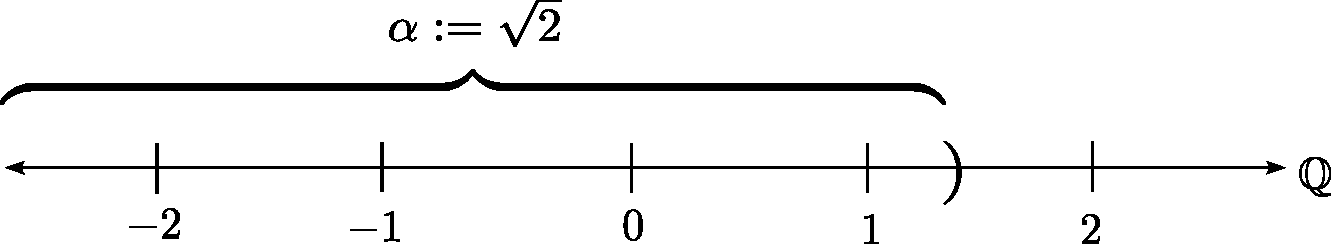
\includegraphics[width=1\linewidth]{figures/sqrt2cut.pdf}
    \caption{The Dedekind Cut corresponding to $\sqrt{2}$}
    \label{fig:enter-label}
\end{figure}
\end{eg}

\begin{theorem}
	$\R$ is an ordered field.
\end{theorem}
\begin{proof}
	 \begin{enumerate}
	     \item $\alpha + \beta := \{r+s: r\in\alpha \text{ and } s\in\beta\}=\beta + \alpha := \{s+r: r\in\alpha \text{ and } s\in\beta\}$, because $\Q$ is a field (and therefore commutative). So, addition in $\R$ commutes.
        \item For $\gamma$ a Dedekind cut, $(\alpha + \beta)+\gamma = \{(s+r)+t: r\in\alpha, s\in\beta\ \text{ and } t\in\gamma\}=\{s+(r+t): r\in\alpha, s\in\beta\ \text{ and } t\in\gamma\} = \alpha + (\beta + 
    \gamma)$ because $\Q$ is a field (and therefore associative). So, addition in $\R$ is associative.
    \item Let $\Q^- =: 0_\R \in\R$. $0_\R + \alpha = \{s+0: s\in\alpha\}= \{s: s\in\alpha\} = \alpha$, so $0_\R$ is an additive identity.
	 \end{enumerate}  \hfill\break
   The remainder of the proof can be found in Baby Rudin.
\end{proof}
\begin{theorem}
	$\R$ satisfies the Axiom of Completeness.
\end{theorem}